\documentclass[11pt,a4paper]{article}

\usepackage[margin=2.6cm]{geometry}
\usepackage[T1]{fontenc}
\usepackage[utf8]{inputenc}
\usepackage{lmodern}
\usepackage{microtype}
\usepackage{amsmath,amssymb,bm}
\usepackage{booktabs}
\usepackage{graphicx}
\usepackage{tabularx}
\usepackage{makecell}
\usepackage{array}
\usepackage[numbers,sort&compress]{natbib}
\usepackage[hidelinks]{hyperref}
\usepackage{url}
\usepackage{xcolor}

\emergencystretch=3em

\newcommand{\X}{\mathbf{X}}
\newcommand{\Y}{\mathbf{Y}}
\newcommand{\A}{\mathbf{A}}
\newcommand{\K}{\mathbf{K}}
\newcommand{\B}{\mathbf{B}}
\newcommand{\Z}{\mathbf{Z}}
\newcommand{\T}{\mathbf{T}}
\newcommand{\R}{\mathbb{R}}
\newcommand{\transpose}{^{\mathsf T}}

\title{\textbf{Reframing preprocessing selection as model-internal calibration in near-infrared spectroscopy}\\
\large A large-scale benchmark of operator-adaptive PLS and Ridge models}

\author{
Gr{\'e}gory Beurier\textsuperscript{1,2}
\quad Robin Reiter\textsuperscript{1,2}
\quad Camille No{\^u}s\textsuperscript{3}\\[0.35em]
Lauriane Rouan\textsuperscript{1,2}
\quad Denis Cornet\textsuperscript{1,2}
}

\date{
\textsuperscript{1}CIRAD, UMR AGAP Institut, Montpellier, France\\
\textsuperscript{2}UMR AGAP Institut, Univ Montpellier, CIRAD, INRAE, Institut Agro, Montpellier, France\\[0.75em]
\textsuperscript{3}Laboratoire Cogitamus, Havre de recherche, \url{https://www.cogitamus.fr/}\\
Camille No{\^u}s: \href{mailto:camille.nous@cogitamus.fr}{camille.nous@cogitamus.fr}\\[0.75em]
Draft of May 13, 2026
}

\begin{document}
\maketitle

\begin{abstract}
Near-infrared spectroscopy (NIRS) is a rapid and non-destructive analytical
technique, but the development of reliable calibration models remains strongly
dependent on spectral preprocessing.  In routine workflows, preprocessing is
commonly selected through large external pipeline searches, which are
computationally costly, statistically unstable on small calibration sets, and
difficult to audit.  Here, we introduce operator-adaptive calibration, a
framework that embeds linear preprocessing selection inside the calibration
model itself.  Candidate spectral treatments are represented as linear
operators acting on the spectra, while nonlinear or sample-adaptive corrections
such as SNV, MSC and ASLS are handled as fold-local branches to avoid leakage.

The framework is instantiated for PLS and Ridge regression.  For PLS, operator
selection is implemented through covariance identities that enable fast NIPALS
and SIMPLS variants while preserving original-wavelength coefficients.  For
Ridge, operator-adaptive kernels provide a dual formulation with recoverable
original-space coefficients.  The approach was evaluated on a heterogeneous
benchmark of more than 50 NIRS datasets and compared with conventional PLS,
Ridge, CatBoost and CNN baselines under documented search budgets.

Compact operator-adaptive PLS combined with ASLS branch preprocessing achieved
a median RMSEP/PLS ratio of 0.960 with 42 wins on 57 datasets, while a
deployable AOM-Ridge selector improved over tuned Ridge by a median 2.22\%
with 35 wins on 52 datasets.  Beyond predictive accuracy, the proposed models
reduce the dependence on large preprocessing-HPO campaigns, produce traceable
operator choices, retain interpretable coefficients, and achieve seconds-scale
fitting for compact AOM-PLS.  Operator-adaptive calibration therefore provides
a practical route toward faster, more robust and auditable NIRS method
development.
\end{abstract}

\noindent\textbf{Keywords:} near-infrared spectroscopy; analytical calibration;
chemometrics; preprocessing selection; partial least squares; ridge
regression; model robustness; spectral data analysis; interpretable machine
learning.

\section{Introduction}

Near-infrared spectroscopy is widely used as a rapid, non-destructive
analytical technique for food, agriculture, plant phenotyping and process
control \citep{burns2007handbook,pasquini2018near}.  Yet the development of
reliable calibration models remains a major bottleneck.  In routine practice,
predictive performance often depends less on the regression algorithm itself
than on the selection of spectral preprocessing.  This selection is usually
performed as an external pipeline search over smoothing, derivatives, scatter
correction, baseline correction and scaling choices.  As a result, calibration
development can become computationally expensive, statistically unstable on
small calibration sets, and difficult to audit.

We argue that preprocessing selection should be treated as a core part of
analytical calibration rather than as an external hyperparameter search.  This
is particularly important for NIRS, where calibration models are frequently
deployed across heterogeneous matrices, traits, instruments and sample sizes.
Preprocessing selection conditions not only predictive performance, but also
external robustness, reproducibility, development cost, transferability to
non-expert users and the auditability of the final calibration object.

The novelty of the present work is therefore not another preprocessing filter.
It is a change in the calibration paradigm: preprocessing alternatives are
treated as structured model components with recoverable coefficients, rather
than as competing black-box pipelines.  We call this approach
operator-adaptive calibration.  Strict linear spectral treatments are encoded
as a bank of operators $\{\A_1,\ldots,\A_m\}$ acting on the spectra, and the
calibration model selects among them internally.  The identity operator is
always included, so standard PLS or Ridge remains available.  Nonlinear or
sample-adaptive corrections such as SNV, MSC and ASLS are kept as explicit
fold-local branches to avoid leakage and to preserve the distinction between
linear operator algebra and fitted preprocessing.

\begin{figure}[t]
  \centering
  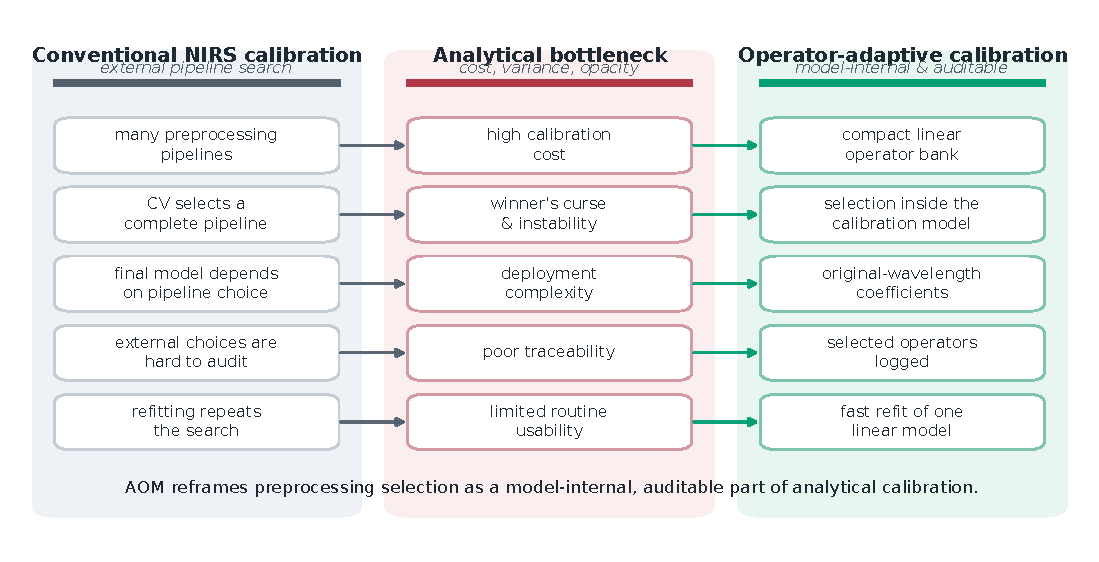
\includegraphics[width=\linewidth]{figures/fig_concept.pdf}
  \caption{From external preprocessing search to operator-adaptive analytical
  calibration.  The proposed workflow converts preprocessing alternatives from
  competing full pipelines into structured model components whose selections
  can be logged, audited and refitted.}
  \label{fig:concept}
\end{figure}

This study makes four contributions to analytical NIRS calibration:
\begin{enumerate}
  \item It introduces operator-adaptive calibration, a framework in which
  linear spectral preprocessing candidates are embedded as model components
  rather than selected as external pipelines.
  \item It provides fast PLS and Ridge instantiations that retain
  original-wavelength coefficients and therefore remain interpretable and
  deployable.
  \item It validates the approach on a heterogeneous benchmark of more than 50
  NIRS datasets, covering diverse sample sizes, response scales and spectral
  structures.
  \item It shows that operator-adaptive calibration can improve predictive
  performance while reducing calibration search complexity and increasing
  traceability.
\end{enumerate}

Unlike many NIRS calibration studies that focus on one matrix or one analytical
trait, we evaluate the proposed strategy across a heterogeneous multi-dataset
benchmark.  This design tests whether the method improves the calibration
process itself, rather than optimizing a single application-specific case.  Our
central claim is that operator-adaptive calibration provides a practical
alternative to large preprocessing-HPO campaigns for NIRS: it improves or
maintains predictive performance across heterogeneous datasets, reduces
calibration search complexity, preserves linear interpretability, and produces
traceable preprocessing decisions suitable for analytical deployment.

\section{Analytical calibration problem and rationale}

\subsection{PLS and Ridge as linear calibration references}

PLS regression constructs latent variables that maximize covariance between
spectra and responses, and has become a standard tool in chemometrics
\citep{geladi1986partial,wold2001pls}.  NIPALS provides an iterative extraction
view, while SIMPLS operates directly on covariance structures
\citep{dejong1993simpls}.  For a centered matrix $\X\in\R^{n\times p}$ and
response $\Y\in\R^{n\times q}$, a PLS model with weights $\mathbf W$,
loadings $\mathbf P$ and response loadings $\mathbf Q$ has regression
coefficients
\begin{equation}
  \B = \mathbf W(\mathbf P\transpose \mathbf W)^+ \mathbf Q\transpose ,
\end{equation}
where $+$ denotes the Moore--Penrose inverse.

Ridge regression estimates a linear coefficient matrix under an $L_2$ penalty
\citep{hoerl1970ridge}.  It is less tied to chemometric tradition than PLS, but
is a strong baseline for high-dimensional collinear predictors because
shrinkage stabilizes the inverse problem.  In dual form, ridge depends on the
sample Gram matrix $\X_c\X_c\transpose$ and is naturally connected to kernel
methods \citep{scholkopf2002learning,hastie2009elements}.

\subsection{Preprocessing as model selection}

Spectral preprocessing aims to reduce nuisance variation or enhance relevant
chemical contrast.  Savitzky--Golay filters smooth spectra and estimate
derivatives \citep{savitzky1964smoothing}; Norris--Williams derivatives are a
related finite-window approach \citep{norris1976influence}.  SNV and MSC reduce
scatter effects \citep{barnes1989standard,geladi1985linearization}, while EMSC
extends this idea with additional terms \citep{martens1991extended}.  Baseline
methods such as asymmetric penalized least squares correct broad low-frequency
drifts \citep{eilers2003perfect,zhang2010baseline}.

These procedures are scientifically meaningful, but their combinations create
a model-selection problem.  A recent local NIRS benchmark protocol used
hierarchical preprocessing search spaces in which PLS and Ridge each evaluated
approximately 5400 candidate fold-level configurations per dataset, CNN-1D
approximately 2700, and CatBoost approximately 90.  Such budgets are defensible
for a benchmark, but they are costly for routine calibration and increase the
risk that the selected pipeline reflects validation noise.

\subsection{Modern baselines}

Gradient boosting methods such as CatBoost \citep{prokhorenkova2018catboost}
and one-dimensional convolutional neural networks
\citep{cui2018modern,mishra2022deep} provide useful nonlinear baselines for
NIRS.  They are valuable comparison points because they represent two common
directions away from classical chemometrics: tabular machine learning and
spectral deep learning.  In this paper they are used as baselines, while the
methodological focus remains on linear, coefficient-bearing calibrations.
Previous work by the authors has also investigated deep learning for NIRS
phenotyping and food-quality traits \citep{vasseur2022perspective,houngbo2024cnn,vaillant2024nirspredict}.

\section{Operator-adaptive calibration framework}

Let $\X\in\R^{n\times p}$ denote spectra and $\Y\in\R^{n\times q}$ denote one
or several responses.  An operator bank is a finite set
\begin{equation}
  \mathcal A = \{\A_1,\ldots,\A_m\}, \qquad \A_b\in\R^{p\times p}.
\end{equation}
Each operator acts on spectra by right multiplication:
\begin{equation}
  \X_b = \X \A_b\transpose .
\end{equation}
The bank contains the identity, ensuring that the unmodified calibration model
is included.  Typical strict linear operators include smoothing matrices,
finite differences, Savitzky--Golay derivatives and detrending projections.

Several selection regimes are possible.  In global selection, one operator is
chosen for the complete model.  In component-wise selection, a different
operator may be selected for each latent component; we treat this
per-operator-per-component variant as exploratory in the present paper because
it can increase selection variance.  In a superblock formulation, all
operator-transformed views are concatenated or combined with weights.  Finally,
nonlinear or sample-adaptive transformations can be placed outside the strict
operator bank as fold-local branches.

The strict linear distinction matters.  Some preprocessing procedures are
linear only after quantities have been estimated from the calibration fold;
others are nonlinear in each sample.  SNV, for example, subtracts and divides
by sample-specific statistics.  MSC and EMSC estimate correction parameters
relative to a reference.  ASLS estimates a baseline through an asymmetric
iterative procedure.  These operations remain useful in chemometric workflows,
but treating them as fixed $\A_b$ matrices would obscure their statistical
role and risk leakage if fitted outside the fold.

\section{Model instantiations}

\subsection{Operator-adaptive PLS}

\subsubsection{Standard PLS notation}

For centered $\X$ and $\Y$, PLS extracts latent scores $\T=\X\mathbf W^*$ and
fits $\Y$ through these scores.  In the notation used here, the coefficient
matrix is
\begin{equation}
  \B = \mathbf W(\mathbf P\transpose \mathbf W)^+ \mathbf Q\transpose ,
\end{equation}
where $\mathbf W$ are weight vectors, $\mathbf P$ are $X$-loadings and
$\mathbf Q$ are $Y$-loadings.  Predictions for new spectra are then
\begin{equation}
  \widehat{\Y} = (\X_{\mathrm{new}}-\bar{\X})\B + \bar{\Y}.
\end{equation}

\subsubsection{Operator-adaptive PLS coefficients}

For a selected operator $\A_b$, a PLS weight vector $r_a$ estimated in the
transformed space corresponds to an original-space effective direction
\begin{equation}
  z_a = \A_b\transpose r_a .
\end{equation}
Collecting these directions in $\Z=[z_1,\ldots,z_k]$ yields scores
\begin{equation}
  \T = \X\Z .
\end{equation}
The original-space coefficient matrix is
\begin{equation}
  \B = \Z(\mathbf P\transpose \Z)^+ \mathbf Q\transpose .
  \label{eq:aompls_coef}
\end{equation}
This is the key interpretability property: even if operators are evaluated
internally, the final model is a single linear map from original spectra to
responses.

\subsubsection{Fast covariance and adjoint implementations}

The materialized reference constructs each $\X\A_b\transpose$ and fits ordinary
PLS.  This is useful for testing but wasteful when many operators are
considered.  For strict linear operators, candidate covariance matrices can be
obtained without materializing transformed spectra:
\begin{equation}
  (\X\A_b\transpose)\transpose\Y = \A_b\X\transpose\Y .
  \label{eq:cov_identity}
\end{equation}
Equation~\ref{eq:cov_identity} directly supports a covariance-space SIMPLS
engine.  A NIPALS implementation can similarly apply adjoint operators to
covariance vectors and then map transformed weights back to original-space
directions.  The implementation used in the experiments includes tests that
identity-only AOM equals standard PLS, fixed-operator materialized and fast
forms agree numerically, and NumPy/PyTorch engines are consistent.

\subsection{Operator-adaptive Ridge}

Ridge regression provides a complementary view because it depends on spectral
geometry rather than on the cross-covariance alone.  Let $\X_c$ and $\Y_c$ be
centered calibration matrices.  For a single operator,
\begin{equation}
  \mathbf Z_b = \X_c\A_b\transpose ,
\end{equation}
and the dual ridge kernel is
\begin{equation}
  \K_b = \mathbf Z_b\mathbf Z_b\transpose
       = \X_c\A_b\transpose\A_b\X_c\transpose .
  \label{eq:ridge_kernel}
\end{equation}
For regularization parameter $\alpha>0$,
\begin{equation}
  \mathbf C = (\K_b + \alpha \mathbf I_n)^{-1}\Y_c ,
\end{equation}
and the original-space coefficient matrix is
\begin{equation}
  \bm\beta_b = \A_b\transpose\A_b\X_c\transpose\mathbf C .
  \label{eq:ridge_beta}
\end{equation}

The superblock case combines several operators by concatenating transformed
blocks with weights $s_b$:
\begin{equation}
  \Phi(\X_c) =
  [s_1\X_c\A_1\transpose \; | \; \cdots \; | \; s_m\X_c\A_m\transpose].
\end{equation}
The resulting kernel is a sum of operator geometries,
\begin{equation}
  \K = \sum_{b=1}^m s_b^2 \X_c\A_b\transpose\A_b\X_c\transpose ,
\end{equation}
and coefficients are recovered as
\begin{equation}
  \bm\beta = \mathbf M \X_c\transpose \mathbf C, \qquad
  \mathbf M = \sum_{b=1}^m s_b^2 \A_b\transpose\A_b .
\end{equation}

This highlights the conceptual difference between the two models.  AOM-PLS
uses the operator action on $\X\transpose\Y$ to select covariance directions.
AOM-Ridge uses the operator action on $\X\X\transpose$ to select a regularized
geometry.  Both remain linear in the original spectra.

\begin{figure}[t]
  \centering
  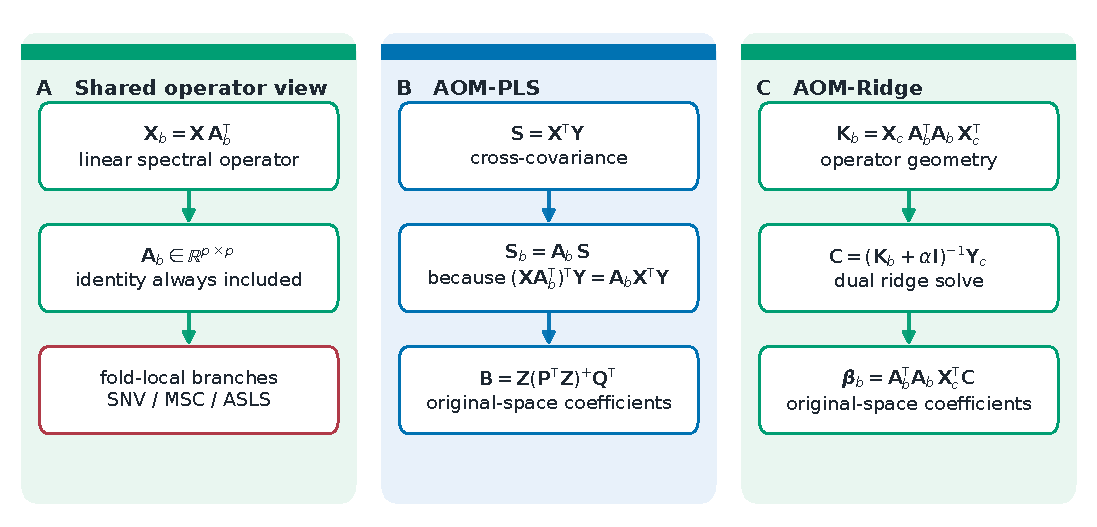
\includegraphics[width=\linewidth]{figures/fig_math.pdf}
  \caption{AOM mathematical structure.  AOM-PLS exploits an operator identity
  on cross-covariances, while AOM-Ridge builds operator-specific sample
  kernels.  Both recover original-space coefficients.}
  \label{fig:math}
\end{figure}

\section{Implementation and software availability}

AOM-PLS and POP-PLS are available in the open-source \texttt{nirs4all} Python
library as regressor and classifier classes for global and component-wise
operator selection.  The same library provides spectral preprocessing,
splitting utilities and pipeline
serialization.  The desktop application \texttt{nirs4all Studio} uses the same
library stack and exposes these workflows through a graphical interface for
users who do not write Python scripts.  The research implementations and
benchmark scripts used for the present AOM-PLS and AOM-Ridge analyses are kept
in the public repository under \texttt{bench/AOM\_v0}.  A clean-room C++
implementation of AOM-PLS is under development to support R bindings and a
dedicated Python package named \texttt{AOM-PLS}.  AOM-PLS and AOM-Ridge are
also planned for pip-distributed implementations once the API and validation
suite are stabilized.  Table~\ref{tab:software} summarizes the current
artifacts.

\begin{table}[t]
  \centering
  \caption{Software availability.  The production package contains the current
  AOM-PLS family; the AOM-Ridge experiments are distributed as research code in
  the benchmark directory pending API stabilization.}
  \label{tab:software}
  \small
  \begin{tabularx}{\linewidth}{p{0.24\linewidth}X X}
\toprule
Artifact & Availability & Role \\
\midrule
\texttt{nirs4all} Python library & \url{https://github.com/GBeurier/nirs4all} & production pipelines, AOM-PLS, POP-PLS, preprocessing, splitting \\
\texttt{nirs4all} documentation & \url{https://nirs4all.readthedocs.io} & user and API documentation \\
\texttt{nirs4all Studio} & \url{https://github.com/GBeurier/nirs4all-webapp} & desktop graphical interface using the same library stack \\
Research benchmark code & repository subdirectory \texttt{bench/AOM\_v0} & AOM-PLS/Ridge experiments, audit tables, scripts \\
\bottomrule
\end{tabularx}

\end{table}

\section{Benchmark design and validation protocol}

\subsection{Datasets and splits}

We used the local multi-dataset NIRS benchmark assembled in the repository.
The benchmark contains heterogeneous regression and classification datasets
covering a wide range of sample sizes, wavelength counts and response scales.
The present paper focuses on regression because AOM-Ridge is currently a
regression method and because the strongest AOM-PLS evidence is regression
based.  Where an original train/test split existed, it was preserved.  When no
external split was provided, deterministic SPXY or stratified variants were
used \citep{kennard1969computer,galvao2005method}.  The external test set was
kept untouched during preprocessing and hyperparameter selection.

\begin{table}[t]
  \centering
  \caption{Benchmark diversity and external-validation design.  The headline
  AOM-PLS and AOM-Ridge claims use different finalized subsets; the table
  reports the corresponding denominators and the broader regression-corpus
  ranges used to characterize heterogeneity.}
  \label{tab:benchmark_diversity}
  \small
  \begin{tabularx}{\linewidth}{p{0.33\linewidth}X}
\toprule
Property & Summary used in this draft \\
\midrule
Headline AOM-PLS cohort & 57 regression datasets in the locked AOM-PLS summary. \\
Headline AOM-Ridge cohort & 52 paired regression datasets after duplicate removal and exclusion of the degenerate QUARTZ reference case. \\
Reference regression corpus & 61 local regression datasets in the AOM benchmark cohort; broader reference table reports 64 regression datasets. \\
Analytical domains & Food and agricultural products, plant and leaf traits, quality traits, fuels, tablets, manure and public NIRS calibration datasets. \\
Sample size range & 40--45,417 samples in the local regression corpus; median 402 samples. \\
Calibration / test size & Calibration sets range from 28 to 39,225 samples; test sets from 12 to 6,192 samples. \\
Spectral variables & 125--4,200 wavelength variables; median 1,023 variables. \\
Dimensional regime & Median $p/n$ approximately 2.38 in the local regression corpus. \\
Split strategy & Original train/test split preserved when available; deterministic SPXY or stratified splitting otherwise. \\
External validation & Test sets are not used for preprocessing, operator, component or regularization selection. \\
\bottomrule
\end{tabularx}

\end{table}

\subsection{Model selection}

For all compared models, preprocessing and hyperparameter selection were
performed inside the calibration set.  PLS selected the number of latent
components by cross-validation.  Ridge selected the regularization parameter
$\alpha$.  CatBoost and CNN-1D followed the local reference benchmark protocol,
with CatBoost using fixed hyperparameters under preprocessing selection and
CNN-1D using a predefined architecture search space.  AOM-PLS selected among
operators in the compact bank and the number of components.  AOM-Ridge selected
operator geometries and regularization in its nested protocol.

The compact AOM operator bank is shown in Table~\ref{tab:operators}.  It is
intentionally small: previous internal experiments found that larger banks can
degrade external-test performance despite improving validation scores, which is
consistent with selection variance and winner's-curse effects in small-$n$
settings.

\begin{table}[t]
  \centering
  \caption{Compact operator bank and branch preprocessing distinction.}
  \label{tab:operators}
  \small
  \input{tables/table_operator_bank.tex}
\end{table}

\subsection{Metrics}

Regression performance is reported primarily through RMSEP on the independent
test set.  Because absolute errors are not comparable across chemical traits
and response scales, dataset-level ratios or relative deltas are used for
aggregate comparisons.  For example, RMSEP/PLS below one indicates improvement
over the PLS reference on the same dataset.  We also report win counts, i.e.,
the number of datasets on which a method has lower RMSEP than the baseline.
Where source tables use percentage deltas, we use
\begin{equation}
  \Delta(\%) = 100 \frac{\mathrm{RMSEP}_{\mathrm{AOM}} -
  \mathrm{RMSEP}_{\mathrm{baseline}}}{\mathrm{RMSEP}_{\mathrm{baseline}}}.
\end{equation}

\subsection{Reference search budgets}

The reference benchmark used a hierarchical preprocessing protocol rather than
an exhaustive unconstrained Cartesian product.  Even with this control, the
linear baselines involve thousands of candidate fold evaluations per dataset:
PLS and Ridge approximately 5400, CNN-1D approximately 2700, and CatBoost
approximately 90.  These counts are important because they clarify what
``baseline performance'' costs in practice.  AOM should therefore be evaluated
not only by RMSEP, but also by the complexity of the calibration procedure that
produces the final model.

\begin{table}[t]
  \centering
  \caption{Search-budget contrast under the local reference benchmark
  protocol.}
  \label{tab:budget}
  \small
  \begin{tabularx}{\linewidth}{p{0.22\linewidth}Xr}
\toprule
Model family & Selection protocol in reference benchmark & Candidate evaluations per dataset \\
\midrule
PLS-HPO & preprocessing hierarchy $\times$ components $\times$ 3 folds & 5400 \\
Ridge-HPO & preprocessing hierarchy $\times$ Optuna trials $\times$ 3 folds & 5400 \\
CatBoost & preprocessing hierarchy with fixed model hyperparameters & 90 \\
CNN-1D & preprocessing hierarchy $\times$ Optuna architecture trials $\times$ 3 folds & 2700 \\
AOM-PLS compact CV-5 & 9-operator compact bank with internal CV selection & seconds-scale fit, median 1.36 s \\
\bottomrule
\end{tabularx}

\end{table}

\section{Results}

\subsection{Large-scale validation across heterogeneous NIRS calibration problems}

The strongest AOM-PLS result in the available full benchmark is the ASLS branch
followed by compact AOM with 5-fold cross-validation.  This variant reaches a
median RMSEP/PLS ratio of 0.960 across 57 datasets, with 42 wins and a median
fit time of approximately 1.36 seconds.  The result has two chemometric
implications.  First, a small bank of interpretable linear operators is enough
to improve over a standard PLS reference on a majority of datasets.  Second,
ASLS remains valuable because baseline correction cannot always be reproduced
by strict fixed linear operators alone.

The deployable AOM-Ridge result is more modest but consistent with the same
calibration principle.  On the 52-dataset paired cohort obtained after
duplicate removal and exclusion of the degenerate QUARTZ reference case, the
Blender selector improves over tuned Ridge by a median 2.22\% and wins on 35
of 52 datasets.  These two deployable results are the primary performance
claims in this draft.

\begin{table}[t]
  \centering
  \caption{Paired statistical summary for the primary deployable comparisons.
  Bootstrap intervals are for the median effect.  Wilcoxon signed-rank tests
  use the one-sided alternative that AOM has lower RMSEP than the reference;
  reported values are Holm-adjusted across the two primary comparisons.}
  \label{tab:paired_stats}
  \small
  \begin{tabularx}{\linewidth}{Xrrrrr}
\toprule
Comparison & $N$ & Median effect & 95\% bootstrap CI & Wins & Wilcoxon $p_{\mathrm{Holm}}$ \\
\midrule
AOM-PLS compact CV-5 vs PLS & 57 & RMSEP ratio 0.960 & 0.926--0.990 & 42/57 & $1.48\times 10^{-4}$ \\
AOM-Ridge Blender vs tuned Ridge & 52 & $\Delta$RMSEP -2.22\% & -3.66 to -0.83\% & 35/52 & $8.05\times 10^{-3}$ \\
\bottomrule
\end{tabularx}

\end{table}

\begin{table}[t]
  \centering
  \caption{Headline benchmark results used in this draft.  Deployable results
  are separated from oracle-envelope values; oracle values quantify headroom
  and do not support deployable performance claims.}
  \label{tab:main_results}
  \small
  \begin{tabularx}{\linewidth}{p{0.30\linewidth}Xrrr}
\toprule
Comparison & Source run & Datasets & Median effect & Wins \\
\midrule
AOM-PLS compact CV-5 vs PLS & full AOM-PLS benchmark & 57 & RMSEP/PLS = 0.960 & 42/57 \\
AOM-Ridge Blender vs Ridge & deployable publication table & 52 & $\Delta$RMSEP = -2.22\% & 35/52 \\
AOM-Ridge AutoSelect vs Ridge & deployable publication table & 52 & $\Delta$RMSEP = -0.61\% & 27/52 \\
AOM-Ridge oracle vs PLS & master-result oracle by class & 58 & RMSEP/PLS = 0.942 & 49/58 \\
AOM-Ridge oracle vs Ridge & oracle publication table & 52 & $\Delta$RMSEP = -4.73\% & 45/52 \\
AOM-Ridge oracle vs CatBoost & oracle publication table & 52 & $\Delta$RMSEP = -13.27\% & 38/52 \\
\bottomrule
\end{tabularx}

\end{table}

\begin{figure}[t]
  \centering
  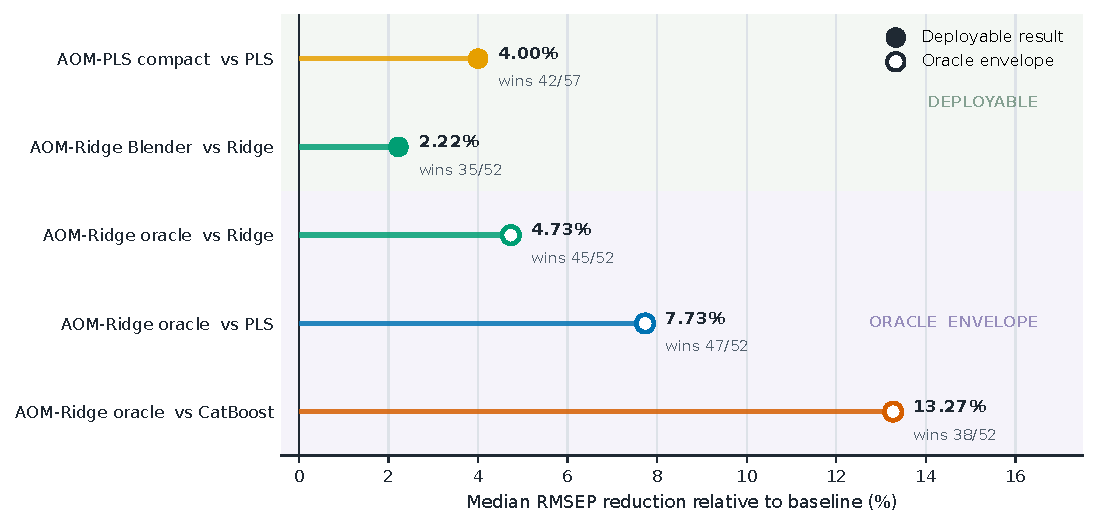
\includegraphics[width=\linewidth]{figures/fig_results.pdf}
  \caption{Median error reductions and win counts from the available headline
  result tables.  Filled markers denote deployable variants; open markers
  denote oracle-envelope analyses.}
  \label{fig:results}
\end{figure}

\subsection{Speed and search-budget reduction}

In analytical method development, calibration cost is not only computational;
it affects how easily a method can be transferred, updated and audited.  A
model requiring thousands of candidate pipeline evaluations may be acceptable
in a benchmark, but is less attractive for routine recalibration.  The proposed
AOM-PLS strategy reduces this burden by replacing a large external
preprocessing search with a compact and structured operator bank.

Figure~\ref{fig:budget} summarizes the search-budget contrast.  The PLS and
Ridge baselines in the reference protocol are not merely single models; they
are selected outcomes of large preprocessing and hyperparameter searches.  By
contrast, compact AOM-PLS evaluates a small structured operator bank and
returns a single original-space linear model with documented selected
operators.  AOM-PLS therefore reaches RMSEP/PLS = 0.960 while replacing
thousands of external preprocessing-HPO evaluations by a compact
operator-adaptive calibration procedure.

\begin{figure}[t]
  \centering
  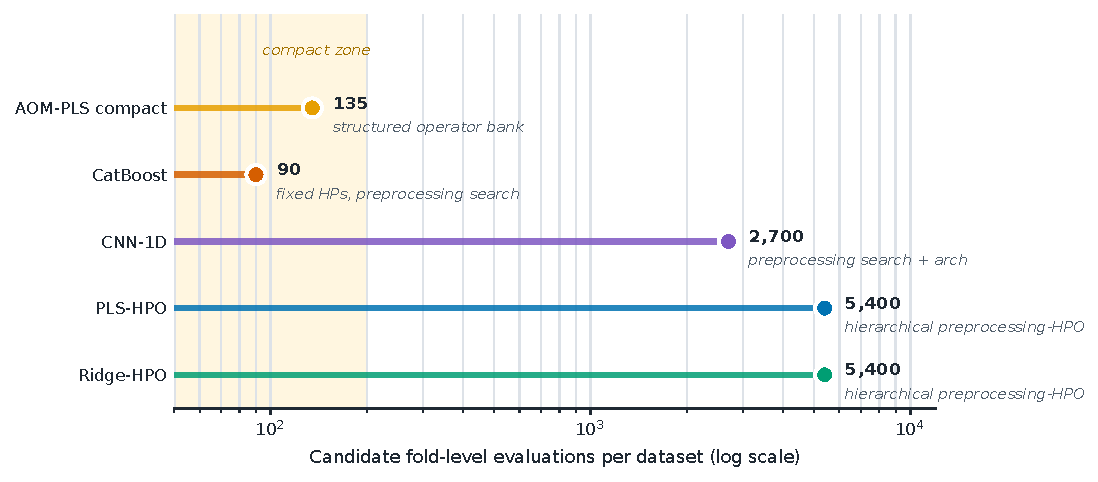
\includegraphics[width=\linewidth]{figures/fig_budget.pdf}
  \caption{Search-budget contrast.  Counts for PLS, Ridge, CatBoost and CNN-1D
  come from the local reference preprocessing-HPO protocol.  The AOM-PLS bar is
  an illustrative compact-bank fold-evaluation count; the measured median fit
  time of the headline compact variant is about 1.36 seconds.}
  \label{fig:budget}
\end{figure}

\subsection{Robustness to preprocessing search complexity}

The ablation pattern is also informative.  Compact banks were more stable than
larger response-deduplicated or family-expanded banks.  Cross-validation
selection was more reliable than a single holdout.  POP-style component-wise
selection and aggressive OSC branches produced interesting individual cases but
were not selected as headline results because they added variance or
instability.  This supports a conservative practical recommendation: start with
identity plus a compact set of smoothing, derivative and detrending operators,
and use nonlinear corrections such as ASLS as explicitly separated branches.

The fact that larger operator banks did not systematically improve
external-test performance is not a weakness of AOM but an important analytical
finding: preprocessing selection is itself a source of model-selection
variance.  Compact operator banks provide a better bias--variance compromise
for routine NIRS calibration because they reduce the number of redundant
candidate filters competing for the same validation signal.

\subsection{Operator-adaptive Ridge as a complementary calibration model}

AOM-Ridge gives a second instantiation of the same operator-adaptive principle.
The strongest deployable variant currently retained in the manuscript is the
Blender selector.  The same result table reports AutoSelect at a median 0.61\%
improvement with 27 wins, and the best single global compact variant at a
median 0.63\% improvement with 29 wins.  This indicates that operator-adaptive
Ridge is promising, but less mature than the compact AOM-PLS pipeline as a
deployment claim.

The stronger AOM-Ridge numbers are oracle-envelope quantities.  In the master
oracle-by-model-class view, AOM-Ridge has a median RMSEP/PLS ratio of
approximately 0.942 and wins on 49 of 58 datasets.  In the 52-dataset
publication-table cohort, the oracle envelope improves over tuned Ridge by a
median 4.73\% and wins on 45 of 52 datasets.  Against PLS, CatBoost and CNN-1D,
the corresponding oracle-envelope median deltas are -7.73\%, -13.27\% and
-12.56\%, respectively.

Oracle results are reported only to quantify the potential headroom of the
operator-kernel formulation and are not used to support deployable performance
claims.  The central point is that Ridge, although less standard than PLS in
routine chemometrics, becomes a useful and interpretable competitor when the
spectral geometry is allowed to adapt through operator kernels.

\section{Analytical implications}

\subsection{What changes for NIRS method development}

The results indicate that a substantial part of NIRS preprocessing selection
can be moved from external pipeline optimization to model-internal calibration
without sacrificing interpretability or predictive performance.  This changes
the practical calibration workflow: analysts can obtain competitive models with
fewer external choices, shorter computation times and a more transparent final
calibration object.

AOM is therefore best viewed as an explicit calibration-layer treatment of a
familiar chemometric choice.  Analysts already know that a derivative, smoother
or detrending step can determine whether a PLS model captures chemistry or
nuisance variation.  AOM preserves this knowledge but expresses it as a bank of
linear operators that can be evaluated inside the model.  This produces a final
linear calibration with inspectable coefficients and a log of selected spectral
operators.

\subsection{Why larger banks can fail}

One might expect that a larger operator bank can only help because it contains
the compact bank as a subset.  That reasoning is valid for calibration
cross-validation minima but not necessarily for external-test performance.
With small calibration sets, many similar operators create multiple
opportunities to overfit validation noise.  The observed superiority of compact
or family-pruned banks is therefore not surprising.  It is an empirical
reminder that preprocessing selection is model selection, and model selection
has variance.

\subsection{PLS and Ridge are complementary}

PLS and Ridge respond differently to operator adaptation.  PLS extracts
supervised latent directions and directly uses cross-covariance with the
response.  Ridge regularizes all spectral directions through shrinkage and
depends on sample geometry.  AOM-PLS is therefore naturally driven by
$\X\transpose\Y$, while AOM-Ridge is driven by $\X\X\transpose$.  In practical
terms, PLS remains the most natural chemometric default, while Ridge becomes a
useful complementary linear model when shrinkage is preferable to latent
variable truncation.

\subsection{Limits of strict linearity}

The strict operator formulation should not be overextended.  SNV, MSC, EMSC
and ASLS are important in NIRS, but their fitted or sample-adaptive nature
requires fold-local handling.  The most successful AOM-PLS result currently
uses ASLS as a branch before compact operator selection, which is a useful
example: the paper does not claim that all preprocessing should be represented
as a fixed matrix.  Rather, fixed linear operators should be integrated where
the algebra is correct, and other procedures should remain explicit pipeline
branches.

\subsection{Implications for routine NIRS calibration}

For routine analytical deployment, the relevant object is not only a benchmark
score but a calibration that can be refitted, inspected and transferred.  AOM
returns a single linear model with coefficients on the original wavelength
grid, records the selected operators, and keeps branch preprocessing inside
the validation workflow.  This is directly aligned with external validation
and with the need to update calibrations when new samples become available.

The value of a method in chemometrics also depends on implementation.  The
AOM-PLS family is available in \texttt{nirs4all} and in \texttt{nirs4all
Studio} \citep{beurier2026nirs4all,beurier2026nirs4allstudio}.  This matters
for adoption because many NIRS users work through graphical pipelines rather
than scripts.  A clean-room C++ implementation of AOM-PLS is being developed
for R and Python distribution under the package name \texttt{AOM-PLS}, and
pip-distributed AOM-PLS/AOM-Ridge implementations are planned once the API and
validation suite are stabilized.  These software routes are part of the
analytical deployment strategy, not only implementation details.

\section{Limitations and future work}

Several limitations should be addressed before journal submission.  First, the
cohort definitions are not yet fully harmonized across all result sources: the
local benchmark contains master tables, AOM-PLS full runs and AOM-Ridge
publication tables with slightly different dataset filters.  A final paper
should freeze one cohort table and regenerate all headline comparisons from
that cohort.  Second, the AOM-Ridge selectors with the best audit evidence
should be promoted through a full 57-dataset, multi-seed nested run before they
are described as production-level defaults.  Third, operator-selection
frequencies and per-dataset failure cases should be added as supplementary
tables.  Fourth, wall-clock comparisons should be measured on the same machine
and reported with hardware details.

For a Talanta submission, the priority experiments are:
\begin{enumerate}
  \item freeze a single regression cohort and rerun the table for PLS-HPO,
  Ridge-HPO, CatBoost, CNN-1D, AOM-PLS compact and AOM-Ridge;
  \item compute paired statistical tests on the common subset, with correction
  for multiple comparisons;
  \item report operator frequencies and selected component counts;
  \item add a no-ASLS strict-linear ablation to quantify how much comes from
  branch baseline correction versus internal operator selection;
  \item add repeated split or multi-seed sensitivity for the strongest
  AOM-Ridge selector.
\end{enumerate}

\section{Conclusion}

Operator-adaptive calibration converts preprocessing selection from an external
trial-and-error pipeline search into an internal, auditable component of the
NIRS calibration model.  For PLS, the covariance identity
$(\X\A_b\transpose)\transpose\Y=\A_b\X\transpose\Y$ enables efficient NIPALS
and SIMPLS implementations while preserving original-space coefficients.  For
Ridge, the same idea becomes a sum of operator-induced geometries in the dual.
On the available heterogeneous NIRS benchmark, compact AOM-PLS and AOM-Ridge
provide competitive linear calibrations with substantially simpler final
models than large preprocessing-HPO workflows.  The practical contribution is
a faster, more traceable and more deployable route for NIRS analytical method
development, especially when calibration must be updated or audited in routine
use.

\section*{Data and Code Availability}

The software is available through \texttt{nirs4all} at
\url{https://github.com/GBeurier/nirs4all} and the documentation at
\url{https://nirs4all.readthedocs.io}.  The desktop application is available at
\url{https://github.com/GBeurier/nirs4all-webapp}.  The AOM research benchmark
materials used for this draft are in the repository under
\texttt{bench/AOM\_v0}, including the AOM-PLS, AOM-Ridge, audit and publication
tables.

\section*{Supplementary Material}

The supplementary material provides the detailed derivations, algorithmic
sketches, evidence-source ledger, deployable/oracle result separation,
leakage-control checklist and experiment backlog required for a full journal
submission.

\section*{Acknowledgements}

This draft was prepared within CIRAD and UMR AGAP Institut.  The authors thank
the developers and users of the \texttt{nirs4all} ecosystem and the teams who
released public NIRS datasets enabling multi-dataset chemometric benchmarking.

\bibliographystyle{unsrtnat}
\bibliography{references}

\end{document}
